\chapter{\ifproject%
\ifenglish Project Structure and Methodology\else โครงสร้างและขั้นตอนการทำงาน\fi
\else%
\ifenglish Project Structure\else โครงสร้างของโครงงาน\fi
\fi
}

\makeatletter

% \renewcommand\section{\@startsection {section}{1}{\z@}%
%                                    {13.5ex \@plus -1ex \@minus -.2ex}%
%                                    {2.3ex \@plus.2ex}%
%                                    {\normalfont\large\bfseries}}

\makeatother
%\vspace{2ex}
% \titleformat{\section}{\normalfont\bfseries}{\thesection}{1em}{}
% \titlespacing*{\section}{0pt}{10ex}{0pt}

\section{หลักการและแนวคิดในการออกแบบ (System Architecture Design)}
\sloppy
การออกแบบระบบตรวจจับและบริหารจัดการคลังสกรูหัวหกเหลี่ยมอัตโนมัติ มีแนวคิดหลักในการนำเทคนิค Image Processing มาประยุกต์ใช้ร่วมกับอุปกรณ์รับภาพและ Web Application เพื่อช่วยตรวจสอบประเภท ขนาด และจำนวนของสกรูหัวหกเหลี่ยม รวมถึงนำผลการตรวจสอบไปใช้ในการบริหารจัดการคลังสินค้า ระบบนี้จะถูกกำหนดให้จำแนกสกรูหัวหกเหลี่ยมได้ทั้งหมด 10 Classes โดยอาศัยคุณลักษณะของวัตถุหลายด้านร่วมกัน เช่น ขนาดและสัดส่วนที่เกี่ยวข้อง เพื่อนำมาใช้จำแนกประเภทของสกรู

\subsection{Data Flow Diagram}

Data Flow Diagram แสดงลำดับการไหลของข้อมูลตั้งแต่ผู้ใช้งานส่งภาพเข้าสู่ระบบ การประมวลผลภาพ การตรวจสอบวัตถุ การจัดเก็บผลลัพธ์ ไปจนถึงการแสดงผลผ่าน Web Application โดยสามารถอธิบายลำดับการทำงานได้ดังนี้

\begin{enumerate}
    \item \textbf{การรับภาพเข้าสู่ระบบ} ผู้ใช้งานสามารถส่งภาพเข้าสู่ระบบได้ 3 รูปแบบ ได้แก่ Real-time Streaming การรับภาพจากกล้องอย่างต่อเนื่อง, Snapshot การบันทึกภาพนิ่งจากกล้องเพื่อนำไปตรวจสอบ และ Upload Image การเลือกไฟล์ภาพจากอุปกรณ์ของผู้ใช้งาน โดยภาพจากทั้งสามรูปแบบจะเข้าสู่กระบวนการตรวจสอบภาพเดียวกัน

    \item \textbf{การส่งภาพผ่าน Web Application และ Backend} เมื่อได้รับภาพแล้ว Web Application จะส่งข้อมูลภาพไปยัง Backend ผ่าน API เพื่อประสานการทำงานกับส่วนประมวลผลภาพ โดย Backend ทำหน้าที่รับข้อมูลและส่งภาพต้นฉบับเข้าสู่กระบวนการประมวลผล

    \item \textbf{การเตรียมภาพก่อนประมวลผล (Image Preprocessing)} ระบบนำภาพที่ได้รับเข้าสู่ขั้นตอนเตรียมภาพ เพื่อให้เหมาะสมกับการตรวจสอบวัตถุ จากนั้นจึงดำเนินการตามกระบวนการ Image Processing ที่กำหนดไว้

    \item \textbf{การตรวจจับและกำหนดกรอบวัตถุ (Visual Inspection)} ผลจากการตรวจจับขอบถูกนำมาใช้ระบุตำแหน่งของวัตถุในภาพ และกำหนดกรอบล้อมรอบวัตถุ (Bounding Boxes) เพื่อแยกวัตถุแต่ละชิ้นออกจากกัน กรอบที่ตรวจพบจะถูกนำไปใช้ในขั้นตอนการวัดขนาดและนับจำนวน ซึ่งการตรวจจับดังกล่าวเป็นการประมวลผลภาพด้วย OpenCV

    \item \textbf{การตรวจสอบและวัดขนาดวัตถุ (Object Inspection and Measurement)} ระบบนำข้อมูลจากกรอบวัตถุที่ตรวจพบมาคำนวณคุณลักษณะต่าง ๆ และพิจารณาคุณลักษณะหลายด้านร่วมกันเพื่อจำแนกประเภทสกรูให้ตรงกับหนึ่งใน 10 Classes ที่กำหนดไว้ การแปลงค่าระยะจาก Pixel เป็นมิลลิเมตรอาศัย Pixel-to-MM Ratio ซึ่งคำนวณจากกระดาษสีขาวขนาด A3 ที่ใช้เป็น Reference ภายในกล่อง จากนั้นระบบนับจำนวนสกรูตามกรอบวัตถุที่ตรวจพบ และสรุปผลการตรวจสอบ

    \item \textbf{การจัดเก็บผลการตรวจสอบ (Database)} Backend รับผลการประมวลผล เช่น ประเภทสกรู ขนาด จำนวน และข้อมูลที่เกี่ยวข้องกับการตรวจสอบ เพื่อนำไปจัดเก็บใน Database โดยข้อมูลภาพจะจัดเก็บเพียง File Path ของภาพไว้ในฐานข้อมูล

    \item \textbf{การเรียกดูและแสดงผล (Result Presentation)} เมื่อ Web Application ต้องการแสดงผล ระบบจะเรียกข้อมูลที่เกี่ยวข้องจาก Backend ซึ่งสามารถดึงข้อมูลผลการตรวจสอบและข้อมูลย้อนหลังจากฐานข้อมูล แล้วส่งกลับไปแสดงบน Web Application ในรูปแบบภาพที่มี Bounding Boxes พร้อมประเภทสกรู ขนาด จำนวน และผลสรุปการตรวจสอบ
\end{enumerate}

\begin{figure}[htbp]
    \centering
    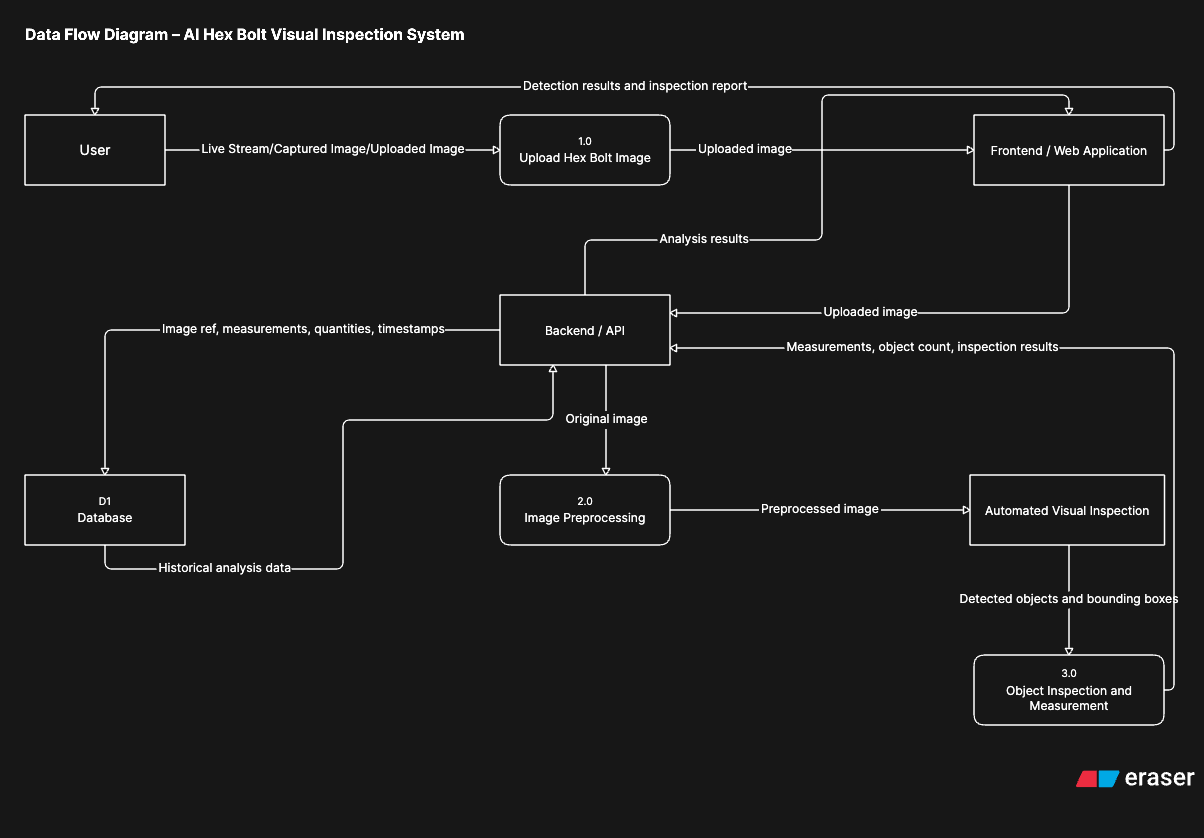
\includegraphics[width=0.95\textwidth]{images/data_flow_diagram.png}
    \caption{Data Flow Diagram ของระบบตรวจจับและบริหารจัดการคลังสกรูหัวหกเหลี่ยมอัตโนมัติ}
    \label{fig:data-flow-diagram}
\end{figure}

\section{Hardware Diagram}

Hardware Diagram แสดงองค์ประกอบของอุปกรณ์ที่ใช้ในการรับภาพและประมวลผล โดยแบ่งออกเป็นส่วนของกล่องควบคุมสภาพแวดล้อมในการถ่ายภาพ อุปกรณ์รับภาพและให้แสงสว่าง และคอมพิวเตอร์สำหรับประมวลผลและใช้งานระบบ ซึ่งมีรายละเอียดดังนี้

\begin{enumerate}
    \item \textbf{กล่องควบคุมสภาพแวดล้อม (Controlled Lighting Box)} กล่องมีขนาด 50 × 40 × 40 เซนติเมตร และมีลักษณะเป็นสีดำเพื่อช่วยป้องกันแสงจากภายนอกรบกวนการถ่ายภาพ ภายในกล่องมีพื้นที่สำหรับวางสกรูและอุปกรณ์ให้แสงสว่าง เพื่อให้สภาพแวดล้อมในการรับภาพมีความสม่ำเสมอมากขึ้น

    \item \textbf{กล้อง Logitech C920e Webcam} ติดตั้งอยู่บริเวณด้านบนของกล่อง โดยหันกล้องลงมายังพื้นที่ตรวจสอบและเชื่อมต่อกับคอมพิวเตอร์โดยตรงผ่าน USB กล้องรองรับความละเอียดสูงสุด 1920 × 1080 พิกเซล มีมุมมองภาพแนวทแยง 78 องศา แนวนอน 70.42 องศา และแนวตั้ง 43.3 องศา ทำหน้าที่รับภาพสำหรับการตรวจสอบทั้งในรูปแบบ Real-time Streaming และ Snapshot

    \item \textbf{LED Ring Light} ติดตั้งอยู่ภายในกล่องเพื่อให้แสงสว่างแก่พื้นที่ตรวจสอบ โดยควบคุมการเปิด-ปิดผ่านสวิตช์แบบ Manual การจัดแสงภายในกล่องมีจุดประสงค์เพื่อลดความแปรปรวนของแสงจากสภาพแวดล้อมภายนอก

    \item \textbf{พื้นที่ตรวจสอบและกระดาษอ้างอิง} ใช้กระดาษสีขาวขนาด A3 ซึ่งมีขนาด 42 × 29.7 เซนติเมตร วางบนพื้นกล่องเป็นพื้นที่สำหรับวางสกรู กระดาษดังกล่าวยังทำหน้าที่เป็น Reference ที่มีขนาดจริงแน่นอน เพื่อใช้คำนวณ Pixel-to-MM Ratio สำหรับแปลงค่าระยะที่วัดได้จากภาพให้เป็นหน่วยมิลลิเมตร

    \item \textbf{คอมพิวเตอร์ (Desktop PC)} ทำหน้าที่รับข้อมูลภาพจากกล้องผ่าน USB และประมวลผลด้วยซอฟต์แวร์ที่พัฒนาขึ้น โดยส่วนประมวลผลภาพใช้ Python และ OpenCV ส่วน Backend ใช้ Node.js และส่วน Web Application ใช้ React, TypeScript และ Vite นอกจากนี้ยังเชื่อมต่อกับ PostgreSQL เพื่อจัดเก็บข้อมูลผลการตรวจสอบและข้อมูลที่เกี่ยวข้องกับคลังสินค้า
\end{enumerate}

ลำดับการทำงานของอุปกรณ์เริ่มจากผู้ใช้งานวางสกรูบนกระดาษ A3 ภายในกล่อง จากนั้นกล้อง Logitech C920e รับภาพและส่งข้อมูลไปยังคอมพิวเตอร์ผ่าน USB โดย LED Ring Light ให้แสงสว่างแก่พื้นที่ตรวจสอบอย่างต่อเนื่อง เมื่อผู้ใช้งานเลือกโหมดการทำงาน ระบบจะรับภาพจากกล้องหรือรับไฟล์ภาพที่อัปโหลด แล้วส่งเข้าสู่กระบวนการประมวลผลภาพเพื่อระบุตำแหน่ง จำแนกประเภท วัดขนาด และนับจำนวนสกรู ผลลัพธ์ที่ได้จะถูกส่งไปยัง Backend เพื่อจัดเก็บในฐานข้อมูลและแสดงผลผ่าน Web Application

\begin{figure}[htbp]
    \centering
    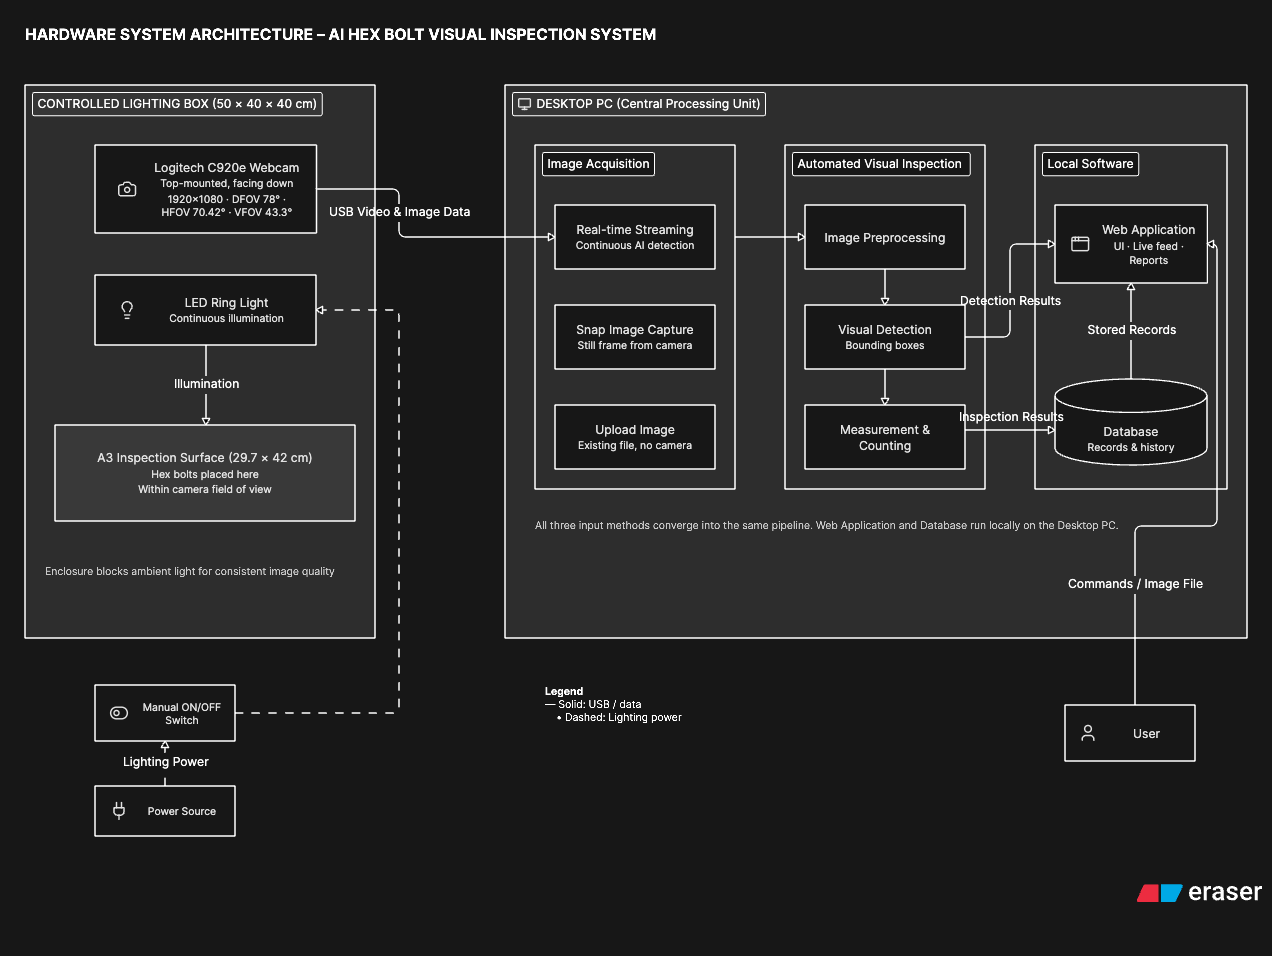
\includegraphics[width=0.95\textwidth]{images/hardware_design.png}
    \caption{Hardware Diagram ของระบบตรวจจับและบริหารจัดการคลังสกรูหัวหกเหลี่ยมอัตโนมัติ}
    \label{fig:hardware-diagram}
\end{figure}

\section{การเตรียมชุดข้อมูลฝึกสอน}

เนื่องจากระบบนี้ใช้เทคนิค Image Processing ด้วย OpenCV จึงไม่มีขั้นตอนการฝึกสอนโมเดลในลักษณะเดียวกับระบบ AI Object Detection อย่างไรก็ตาม จำเป็นต้องเตรียมภาพตัวอย่างของสกรูแต่ละประเภทเพื่อใช้เป็นข้อมูลอ้างอิงในการพัฒนาและปรับค่าพารามิเตอร์ของกระบวนการประมวลผลภาพ รวมถึงใช้ตรวจสอบความเหมาะสมของคุณลักษณะที่นำมาใช้จำแนกประเภทสกรู

ภาพตัวอย่างจะเก็บจากการถ่ายภาพสกรูภายในกล่องควบคุมสภาพแวดล้อม โดยใช้กล้อง Logitech C920e และจัดวางสกรูบนกระดาษสีขาวขนาด A3 เพื่อควบคุมพื้นหลังและใช้เป็น Reference สำหรับคำนวณ Pixel-to-MM Ratio
ประเภทสกรูที่กำหนดไว้สำหรับระบบประกอบด้วย 10 Classes ดังนี้

\begin{enumerate}
    \item M6 × 70 mm
    \item M20 × 50 mm
    \item M12 × 100 mm
    \item M10 × 60 mm
    \item 1/2 × 2"
    \item 3/8 × 1½"
    \item M14 × 65 mm
    \item 5/8 × 2"
    \item M8 × 80 mm
    \item 3/8 × 3"
\end{enumerate}

ในการใช้งานจริง ภาพหนึ่งภาพสามารถมีสกรูได้หลายชิ้นและอาจมีสกรูหลายประเภทพร้อมกัน โดยมีเงื่อนไขว่าสกรูแต่ละชิ้นต้องไม่ซ้อนทับกัน และต้องอยู่ภายในขอบเขตของกระดาษอ้างอิง เพื่อให้ระบบสามารถตรวจจับกรอบวัตถุและวัดขนาดได้อย่างเหมาะสม

\section{การพัฒนา Web Application}

Web Application ถูกพัฒนาขึ้นเพื่อเป็นส่วนติดต่อระหว่างผู้ใช้งานกับระบบตรวจสอบสกรูและระบบบริหารจัดการคลังสินค้า โดยแบ่งการพัฒนาเป็นส่วน Frontend, Backend และ Image Processing เพื่อแยกหน้าที่การทำงานและให้แต่ละส่วนสามารถสื่อสารกันผ่านการรับส่งข้อมูลได้

ส่วน Frontend พัฒนาด้วย React ร่วมกับ TypeScript และ Vite ทำหน้าที่แสดงหน้าจอการใช้งาน รับคำสั่งจากผู้ใช้งาน และแสดงผลการตรวจสอบ ส่วน Backend พัฒนาด้วย Node.js ทำหน้าที่รับส่งข้อมูลระหว่าง Frontend กระบวนการประมวลผลภาพ และฐานข้อมูล ขณะที่การประมวลผลภาพดำเนินการด้วย Python และ OpenCV เมื่อได้ผลการตรวจสอบแล้ว Backend จะนำข้อมูลไปจัดเก็บใน PostgreSQL และส่งผลลัพธ์กลับไปยัง Frontend เพื่อแสดงผล

ระบบรองรับการรับภาพ 3 รูปแบบ ได้แก่ Real-time Streaming สำหรับรับและประมวลผลภาพจากกล้องทุก Frame อย่างต่อเนื่อง, Snapshot สำหรับบันทึกภาพนิ่งจากกล้องแล้วส่งไปประมวลผล และ Upload Image สำหรับเลือกไฟล์ภาพจากภายนอกเข้าสู่ระบบ โดยทั้งสามรูปแบบใช้กระบวนการตรวจสอบภาพเดียวกัน

\subsection{UX/UI}

การออกแบบ UX/UI เริ่มจากการออกแบบหน้าจอและลำดับการใช้งานด้วย Figma ก่อนนำไปพัฒนาเป็น Web Application โดยมุ่งเน้นให้ผู้ใช้งานสามารถตรวจสอบสกรู ดูผลการวิเคราะห์ และจัดการข้อมูลคลังสินค้าได้จากระบบเดียว หน้าจอหลักที่กำหนดไว้มีดังนี้

\begin{enumerate}
    \item \textbf{หน้าตรวจสอบสกรู (Inspection)} เป็นหน้าสำหรับรับภาพและแสดงผลการตรวจสอบ ผู้ใช้งานสามารถเลือกอุปกรณ์กล้อง ตรวจสอบสถานะอุปกรณ์ และควบคุมการเปิด-ปิดกล้องหรือ LED ได้ตามที่ระบบรองรับ นอกจากนี้ยังสามารถเลือกโหมด Real-time, Snapshot หรือ Upload Image ได้ เมื่อระบบประมวลผลเสร็จจะแสดงภาพที่มีกรอบ Bounding Boxes พร้อมประเภทสกรู ขนาด จำนวน และผลรวมของการตรวจสอบ รวมถึงมีส่วนสำหรับดำเนินการเพิ่มหรือลดจำนวนสินค้าในคลังจากผลการตรวจสอบ

    \item \textbf{หน้าคลังสินค้า (Inventory)} เป็นหน้าสำหรับแสดงข้อมูลสินค้าและจำนวนคงเหลือในคลัง ผู้ใช้งานสามารถดูภาพรวมของคลังสินค้า ค้นหาและกรองข้อมูล รวมถึงจัดการข้อมูลสินค้าและจำนวนสต๊อก โดยรองรับการเพิ่มสินค้า การลดจำนวนสินค้า การแก้ไขข้อมูล และการลบข้อมูล

    \item \textbf{หน้าประวัติการใช้งาน (History)} เป็นหน้าสำหรับเรียกดูประวัติการตรวจสอบและรายการเปลี่ยนแปลงข้อมูลคลังสินค้า โดยข้อมูลที่แสดงประกอบด้วยวันที่ตรวจสอบ ประเภทสกรู จำนวนที่ตรวจพบ และผลการวิเคราะห์ รวมถึงประวัติการดำเนินการ เช่น การเพิ่มหรือการลดจำนวนสินค้า ผู้ใช้งานสามารถค้นหาและกรองข้อมูล รวมถึงส่งออกข้อมูลประวัติในรูปแบบ CSV ได้
\end{enumerate}

\subsection{การจัดการฐานข้อมูล}

ระบบใช้ PostgreSQL เป็นระบบจัดการฐานข้อมูลสำหรับจัดเก็บข้อมูลที่เกี่ยวข้องกับผลการตรวจสอบและการบริหารจัดการคลังสินค้า โดยข้อมูลภาพจะจัดเก็บเป็นไฟล์แยกจากฐานข้อมูล และบันทึกตำแหน่งที่จัดเก็บไฟล์ (File Path) ไว้ใน PostgreSQL เพื่อให้ระบบสามารถอ้างอิงและเรียกใช้ภาพที่เกี่ยวข้องกับผลการตรวจสอบได้

ข้อมูลที่ระบบจำเป็นต้องจัดเก็บในภาพรวมประกอบด้วยข้อมูลประเภทสกรู ข้อมูลจำนวนสินค้าในคลัง ผลการตรวจสอบ และประวัติการเปลี่ยนแปลงข้อมูล เช่น การเพิ่มหรือการลดจำนวนสินค้า รวมถึงข้อมูลวันที่และรายละเอียดที่เกี่ยวข้องกับการตรวจสอบ อย่างไรก็ตาม ในขั้นตอนการจัดทำรายงานนี้ โครงสร้างตาราง ความสัมพันธ์ระหว่างตาราง และรายละเอียดของ Database Schema ยังอยู่ระหว่างการออกแบบ จึงยังไม่ระบุชื่อ Table หรือโครงสร้าง Field ที่แน่นอน